\documentclass[a5paper]{article}
\usepackage[a5paper, top=8mm, bottom=8mm, left=8mm, right=8mm]{geometry}

\usepackage{polyglossia}
\setdefaultlanguage[babelshorthands=true]{russian}

\usepackage{fontspec}
\setmainfont{FreeSerif}
\newfontfamily{\russianfonttt}[Scale=0.7]{DejaVuSansMono}

\usepackage[font=scriptsize]{caption}

\usepackage{amsmath}
\usepackage{amssymb,amsfonts,textcomp}
\usepackage{color}
\usepackage{array}
\usepackage{hhline}
\usepackage{cite}

\usepackage[hang,multiple]{footmisc}
\renewcommand{\footnotelayout}{\raggedright}

\PassOptionsToPackage{hyphens}{url}\usepackage[xetex,linktocpage=true,plainpages=false,pdfpagelabels=false]{hyperref}
\hypersetup{colorlinks=true, linkcolor=blue, citecolor=blue, filecolor=blue, urlcolor=blue, pdftitle=1, pdfauthor=, pdfsubject=, pdfkeywords=}

\usepackage{tabu}

\usepackage{graphicx}
\usepackage{indentfirst}
\usepackage{multirow}
\usepackage{subfig}
\usepackage{footnote}
\usepackage{minted}

\sloppy
\pagestyle{plain}

\title{Визуальное моделирование, UML}
\author{Юрий Литвинов\\\small{yurii.litvinov@gmail.com}}

\date{24.04.2020г}

\begin{document}

\maketitle
\thispagestyle{empty}

\section{Введение}

Как известно, при разработке ПО много времени требуется на анализ и проектирование. Если просто сесть и начать писать код, ничего хорошего из этого не выйдет. Для реализации программ есть удобные формализмы --- различные языки программирования, методологии и технологии. Для анализа и проектирования языки программирования, как правило, не годятся, поскольку требуют слишком детального изложения решения задачи. Там применяются свои специальные методики, например, при разработке алгоритмов --- псевдокод или блок-схемы. Блок-схемы на самом деле не используются уже давно, и по ходу дальнейшего изложения вы поймёте, почему.

Подавляющее большинство разрабатываемых приложений гораздо сложнее просто реализации алгоритма, поэтому нужно уметь выделять наиболее существенную информацию об архитектуре системы. Такое представление существенной информации без деталей реализации и называется моделью системы. Наиболее удобными и наглядными являются визуальные модели, где информация об архитектуре системы представляется в виде диаграмм. Наиболее близким аналогом визуальных моделей ПО в ``обычной'' инженерии являются чертежи --- так же, как здание строится по нарисованным архитектором чертежам, так и крупные приложения программируются по нарисованным архитектором визуальным моделям. Кроме того, визуальные модели применяются не только при проектировании, но и при общении между программистами --- гораздо проще показать картинку, по которой всё понятно, чем кучу кода, и при общении с заказчиком --- заказчик вообще программировать может не уметь, а если показать картинку, ему после краткого объяснения нотации всё сразу станет понятно. Ну и по тем же причинам диаграммы --- хорошее средство для документации. Ещё есть мнение, что диаграммы должны быть такими, чтобы по ним можно было сгенерировать исполняемый код --- не пропадать же уже нарисованным диаграммам. Это спорно, потому что для генерации кода диаграммы должны содержать все необходимые детали, что противоречит самой сути моделирования --- упрощению системы. Модель всегда должна быть проще того, что она моделирует, иначе в ней нет никакого смысла. Впрочем, программирование диаграммами (или визуальное программирование) вполне имеет право на жизнь и даже местами применяется, но слово ``моделирование'' при таком подходе неуместно.

Визуальные модели и чертежи имеют одно принципиальное отличие, вытекающее из принципиального отличия объектов физического мира и программ --- программное обеспечение невидимо. Здание, деталь, подводную лодку можно нарисовать, так, как мы увидим её глазами (или похоже), программное обеспечение мы не видим. Мы видим текст программы, видим внешние проявления работы программы, но это не сама программа. Как выглядит программа, вообще говоря, непонятно. Поэтому рисовать программные системы можно весьма по-разному. Поэтому любая визуализация программного обеспечения представляет собой некоторую метафору --- некоторые абстрактные и невидимые сущности программной системы сопоставляются видимым человеческому глазу объектам, всяким квадратикам и кружочкам. В общем-то, точно так же, эти абстрактные сущности сопоставляются тексту на конкретном языке программирования, или даже словесному описанию --- это лишь разные способы передать информацию об одном объекте. Из этих соображений, и ещё из того, что модель должна представлять только существенную информацию, следует ещё одно важное для визуального моделирования понятие: точка зрения моделирования. Визуальная модель всегда направлена на конкретную группу читателей, и служит конкретно для чего-то, не бывает просто визуальных моделей. Визуальные модели бывают трёх типов --- одноразовые, служащие исключительно для коммуникации, нарисовали диаграмму, потыкали в неё пальцами, изложили мысль и выкинули, документация --- такая модель, которую можно положить в гит или даже повесить на стенку (последний вариант бывает полезен при разработке больших систем, вешаем на стенку диаграмму с высокоуровневой архитектурой системы и стараемся ей следовать при разработке и сопровождении), и диаграммы, по которым генерируется код, фактически, графические исходники. Когда вы рисуете диаграмму, вы должны чётко понимать, зачем вы её рисуете. Если вы хотите объяснить кому-то идею решения задачи, вы рисуете только то, что существенно для объяснения, причём для объяснения именно того, что вы хотите объяснить, и именно тому, кому вы объясняете (картинки для директора и для вашего коллеги-программиста могут быть совсем разные).

Например, идея решения задачи про хеш-таблицы со сменными хеш-функциями может быть выражена такой моделью:

\begin{center}
	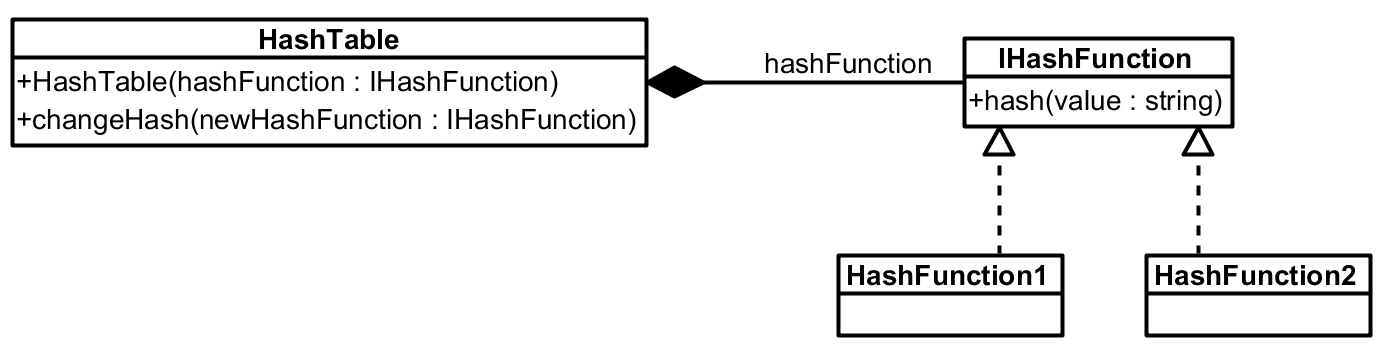
\includegraphics[width=0.9\textwidth]{modelExample.png}
\end{center}

Понятно, что у хеш-таблицы ещё куча методов, что она содержит ещё массив списков и всё такое, но к делу это имеет слабое отношение, а идея решения по этой диаграмме более-менее понятна: мы заводим интерфейс для хеш-функции, реализуем его в классах --- настоящих хеш-функциях, и передаём объекты этих классов конструктору хеш-таблицы, или специальному методу смены хеш-функции.

Понятно, что если рисовать диаграммы уж совсем абы как, от них будет мало пользы в деле передачи информации, потому что у каждого свои представления о том, как выглядит ПО. Требуется некая общепризнанная унифицированная нотация, чтобы незнакомые люди могли обмениваться диаграммами и однозначно понимать, что именно нарисовано. Такой нотации до 1996 года не было, была куча конкурирующих визуальных нотаций. В 1996 году авторов трёх наиболее популярных из них собрали вместе и велели ругаться, пока они не выработают единую нотацию. В результате они смогли договориться, так появился язык визуального моделирования UML. Та диаграмма, которая показана выше --- это пример диаграммы классов UML. Язык UML описывает довольно большое количество различных видов диаграмм (сейчас 13 штук), которые служат для описания программной системы с различных точек зрения --- высокоуровневая структура системы (из каких компонентов она состоит), более низкоуровневая структура (из каких классов состоит система и как эти классы взаимосвязаны), поведение системы, что делает система, как система располагается на физическом оборудовании, как организован обмен сообщениями в различных частях системы, как меняется состояние частей системы в зависимости от времени, и т.д. Диаграммы в UML делятся на две группы --- структуры (описывающие статическую структуру программы) и поведения (описывающие различные аспекты поведения системы во время выполнения). Вот диаграмма, показывающая отношения между диаграммами UML:

\begin{center}
	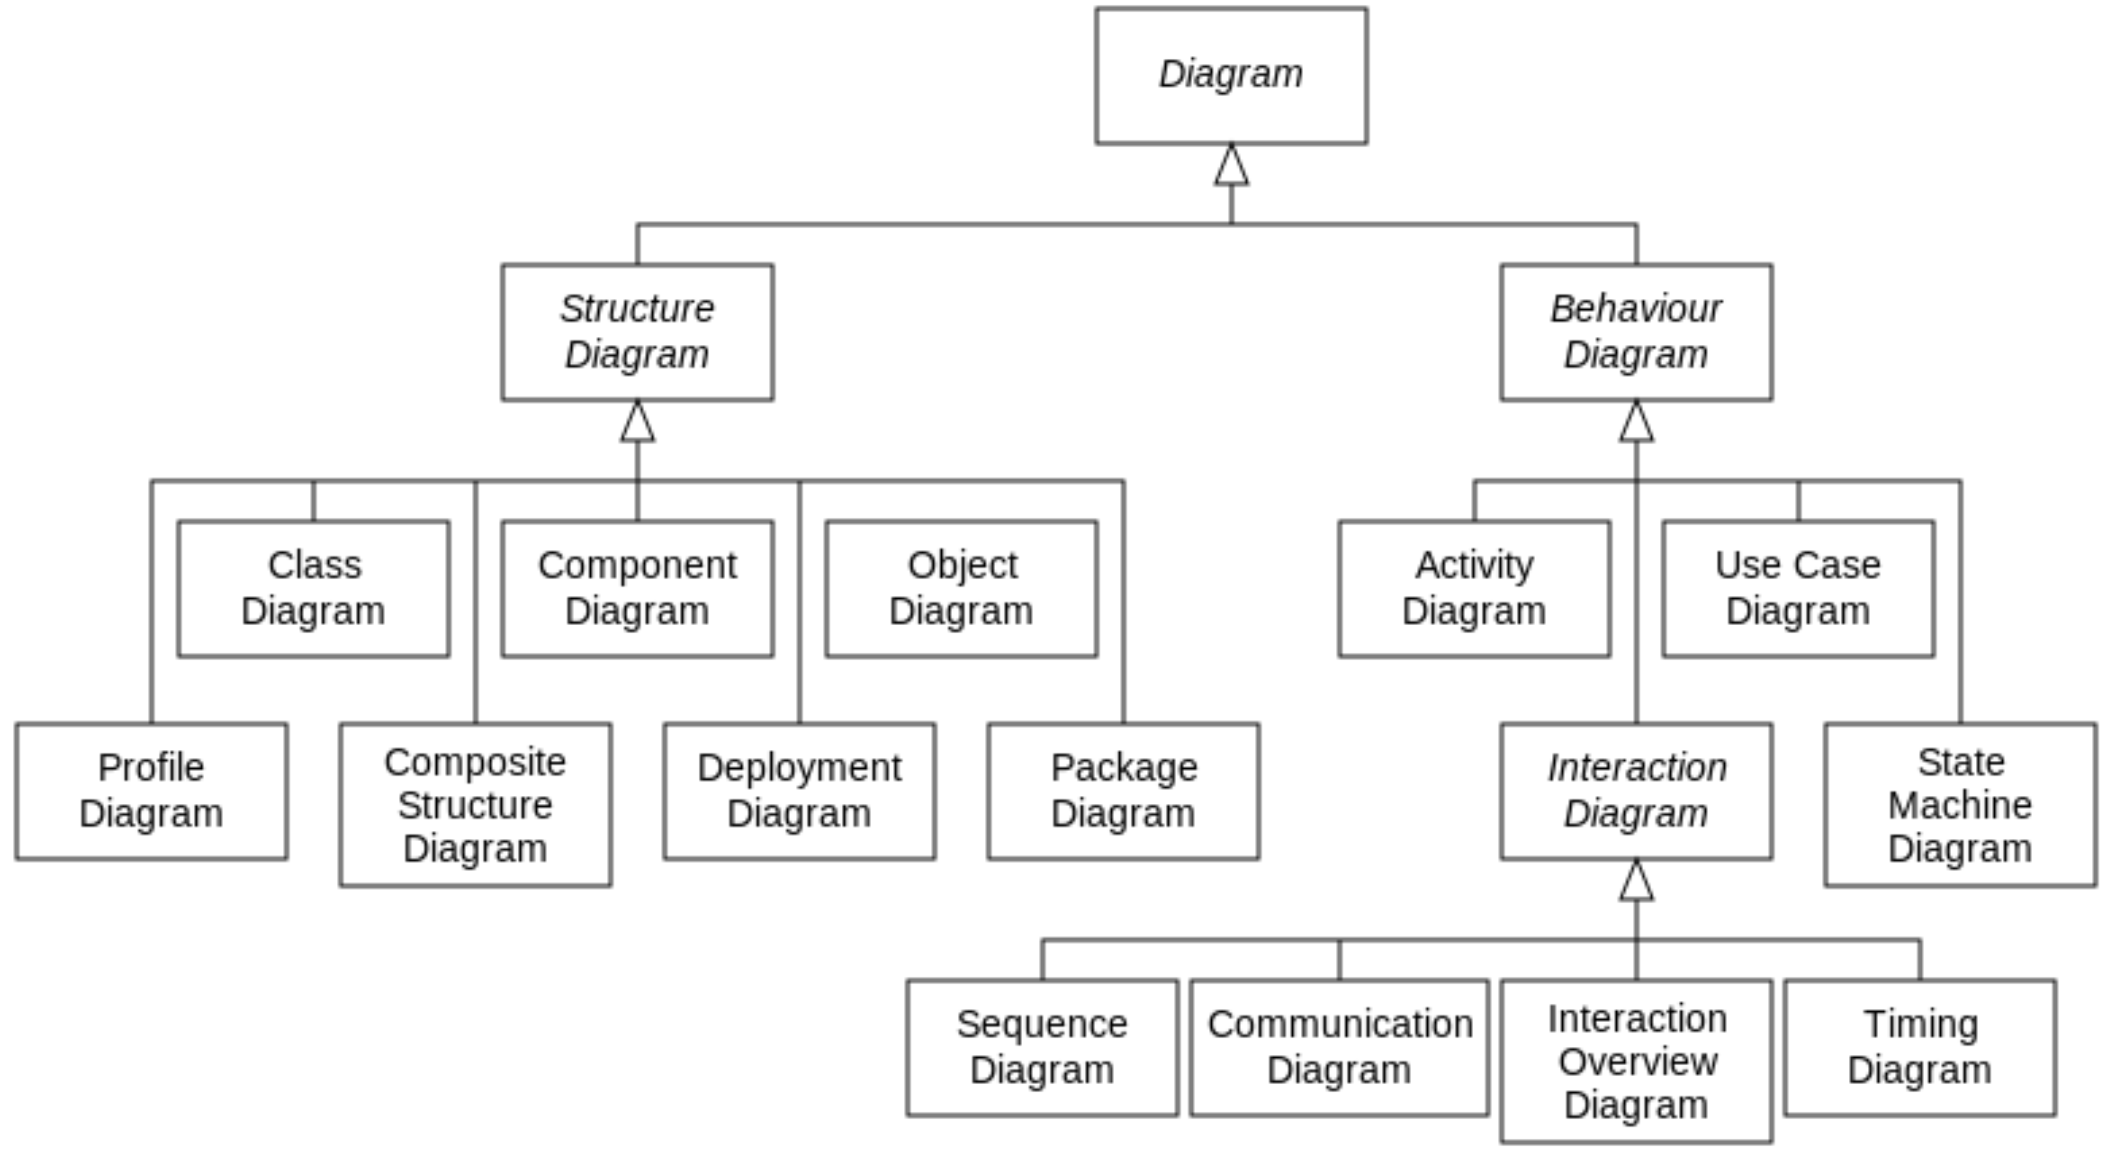
\includegraphics[width=0.9\textwidth]{umlDiagrams.png}
\end{center}

\section{Диаграммы классов}

Самая широко применяемая диаграмма UML --- это диаграмма классов. Диаграмма классов описывает типы объектов системы и различного рода статические отношения между ними. Там рисуются классы с полями и методами, и связи, которые могут быть между объектами этих классов. Вот картинка с синтаксисом диаграммы:

\begin{center}
	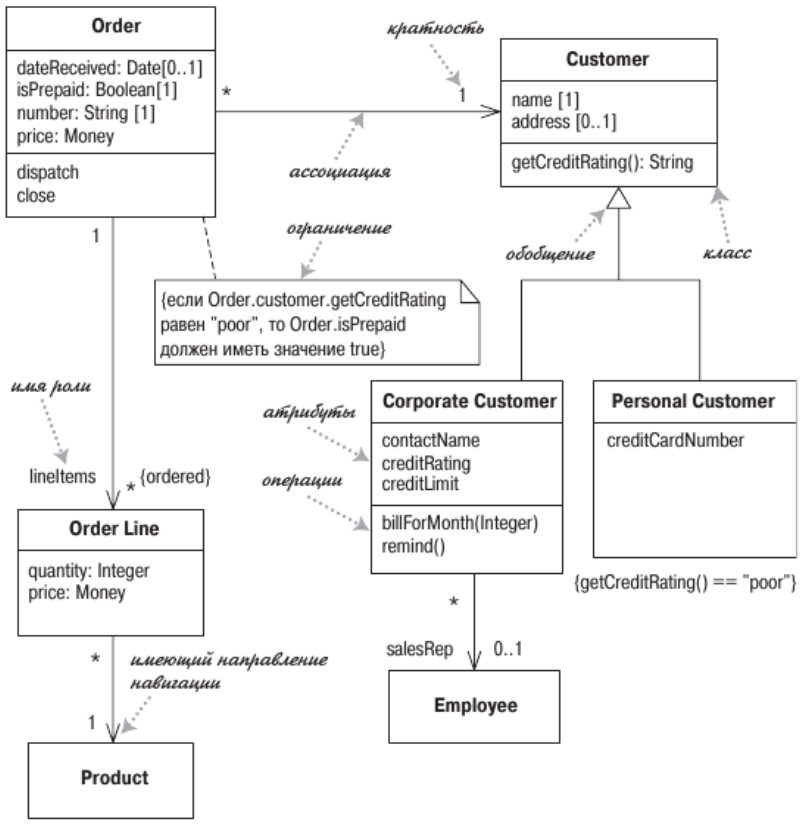
\includegraphics[width=0.7\textwidth]{umlClassDiagram.png}
\end{center}

В общем случае объявление поля выглядит как ``видимость имя: тип кратность = значение по умолчанию {строка свойств}''. Обязательно только имя. Видимость бывает + (public), - (private), \# (protected), \textasciitilde (package). Кратность может задаваться в виде 1 (ровно 1 объект), 0..1 (ни одного или один), * (сколько угодно), можно 1..*, можно 2..*. Поле не обязательно описывать как, собственно, поле, его можно изобразить в виде ассоциации, как показано на картинке выше, например, у товара может быть несколько строк заказа, тогда как каждой строке заказа соответствует один товар. Ассоциации могут иметь направление (направление навигации), показывающее, какой класс о каком знает, ассоциация может быть двунаправленной, если направление не задано, то либо ассоциация двунаправленная, либо направление на данном уровне моделирования просто не важно. Статические поля и методы рисуются подчёркнутыми.

Ещё можно явно указать тип ассоциации:

\begin{center}
	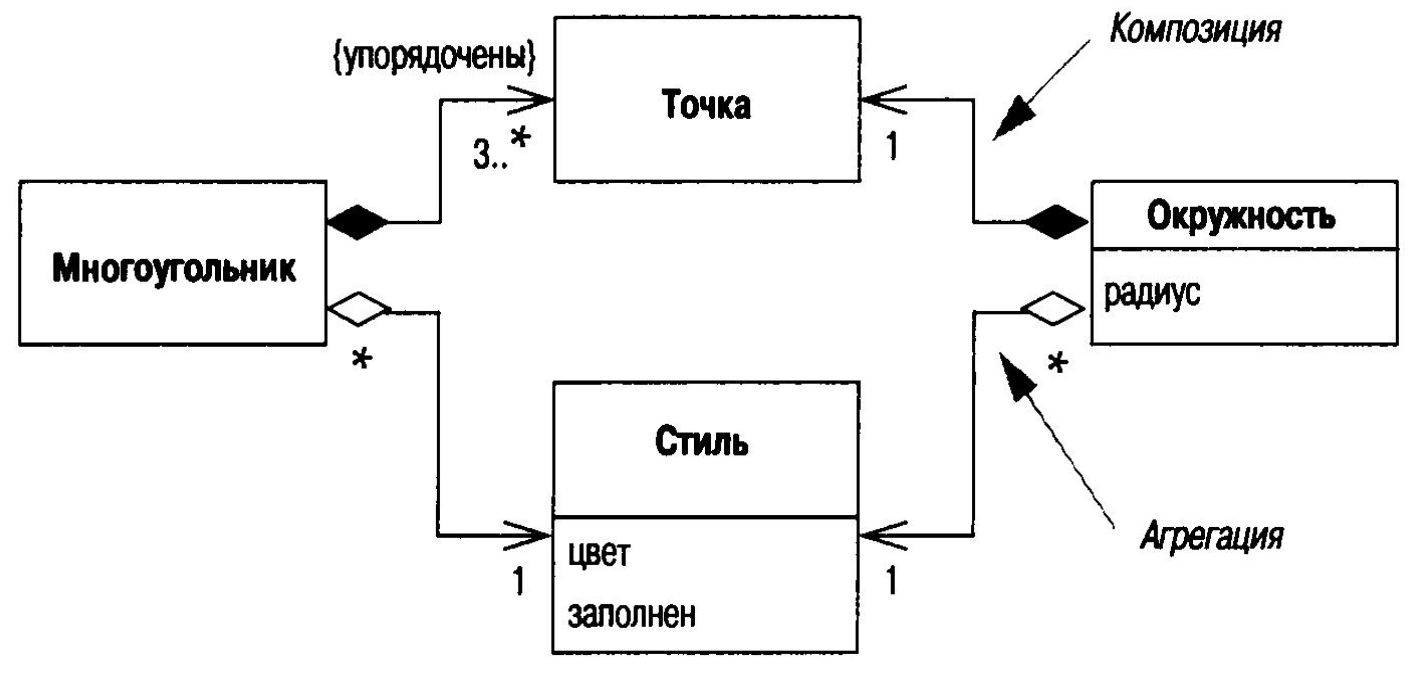
\includegraphics[width=0.6\textwidth]{associationTypes.png}
\end{center}

Бывают ассоциации агрегации и композиции. Агрегация, как правило, это отношение, показывающее, что один объект знает о другом и может инициировать с ним взаимодействие. Композиция задаёт отношение владения --- экземпляр класса, участвующего в композиции, может иметь только одного объекта-владельца, несмотря на то, что сам класс может участвовать в нескольких отношениях композиции. Агрегация же говорит, что класс просто знает о другом классе, но не владеет им. Например, на картинке точка может быть либо вершиной многоугольника, либо центром окружности, но не и тем и другим одновременно. Тогда как стиль для всех объектов может быть один. Важно помнить, что объекты,  связанные отношением композиции с объектом-владельцем, не могут жить отдельно от него, так что когда его удаляют, они удаляются вместе с ним. Поэтому отношение композиции показывает свойства, которыми владеют по значению (это весьма важно для С++ и не так существенно для C\# или Java --- в C\# и Java есть сборка мусора, а вот в С++ ясное понимание отношений владения нужно для управления памятью). Агрегация и композиция являются частными случаями ассоциации, так что допустимо на более высокоуровневых диаграммах рисовать их как просто ассоциации, а когда это становится важным (ближе к реализации) --- специфицировать, что именно за ассоциацию мы имеем в виду.

Интерфейсы и абстрактные классы рисуются вот так:

\begin{center}
	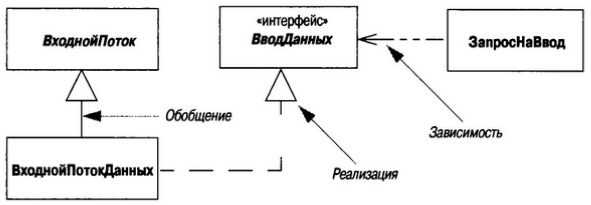
\includegraphics[width=0.7\textwidth]{interfaces1.png}
\end{center}

Имена абстрактных классов пишутся курсивом, интерфейсов --- тоже, но ещё и с <<interface>>. Реализация и зависимость (то есть использование интерфейса) --- на картинке понятно как. Обобщение ещё называют генерализацией, это отношение наследования. Можно рисовать интерфейсы ещё и так:

\begin{center}
	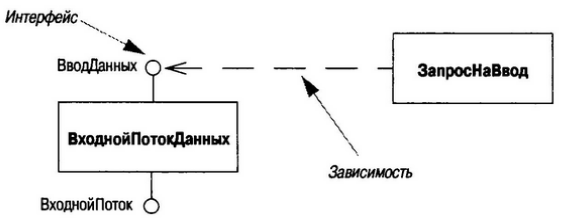
\includegraphics[width=0.6\textwidth]{interfaces2.png}
\end{center}

Такая нотация обычно применяется для достаточно крупных частей системы, например, для компонентов.

Можно даже генерики рисовать:

\begin{center}
	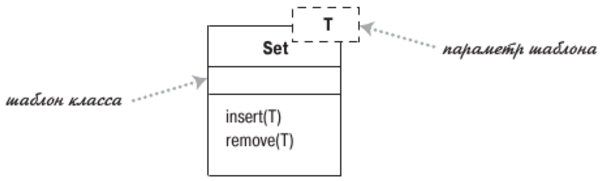
\includegraphics[width=0.7\textwidth]{templates.png}
\end{center}

Комментарии рисуются так:

\begin{center}
	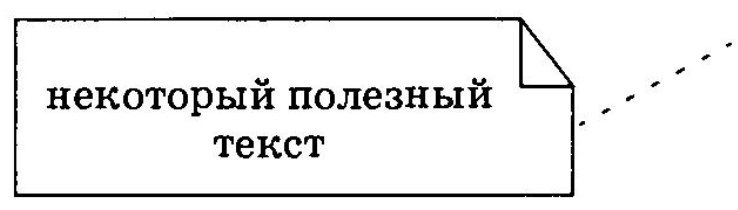
\includegraphics[width=0.4\textwidth]{comment.png}
\end{center}

Цепляются пунктирной линией к тому, что они комментируют. Комментарии можно рисовать не только на диаграмме классов, но и где угодно. Можно их ни с чем не связывать, тогда это будет комментарий к диаграмме вообще.

\section{Диаграммы активностей}

Следующая весьма распространённая диаграмма --- это диаграмма активностей (или диаграммы деятельности). Они служат для описания поведения системы. То есть, на самом деле, их предназначение --- моделирование бизнес-процессов и потоков работ, но они вполне могут использоваться и для описания поведения методов. Выглядят они вот так:

\begin{center}
	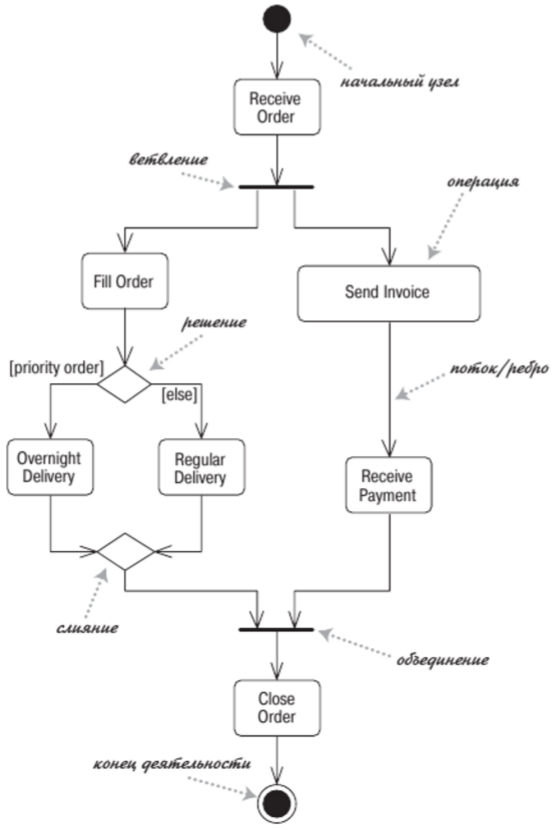
\includegraphics[width=0.7\textwidth]{activityDiagram.png}
\end{center}

 - очень похоже на блок-схему, однако же, имеет нотацию для параллельного исполнения и другие вещи, которых в классических блок-схемах нет. Обычно такими диаграммами моделируются процессы, происходящие в реальном мире, где в итоге должна будет работать создаваемая система, для лучшего понимания её окружения. Ещё такими диаграммами можно описывать высокоуровневое поведение системы --- что именно она делает и в какой последовательности. Ещё можно такими диаграммами специфицировать реализацию каждого конкретного метода каждого класса, составляющего систему, но толку от таких диаграмм мало, потому что код в текстовом виде вполне может оказаться понятнее (такие диаграммы имеют свойство быстро расти в размерах и сложности). Действия на диаграмме могут сами раскрываться в поддиаграммы:

\begin{center}
	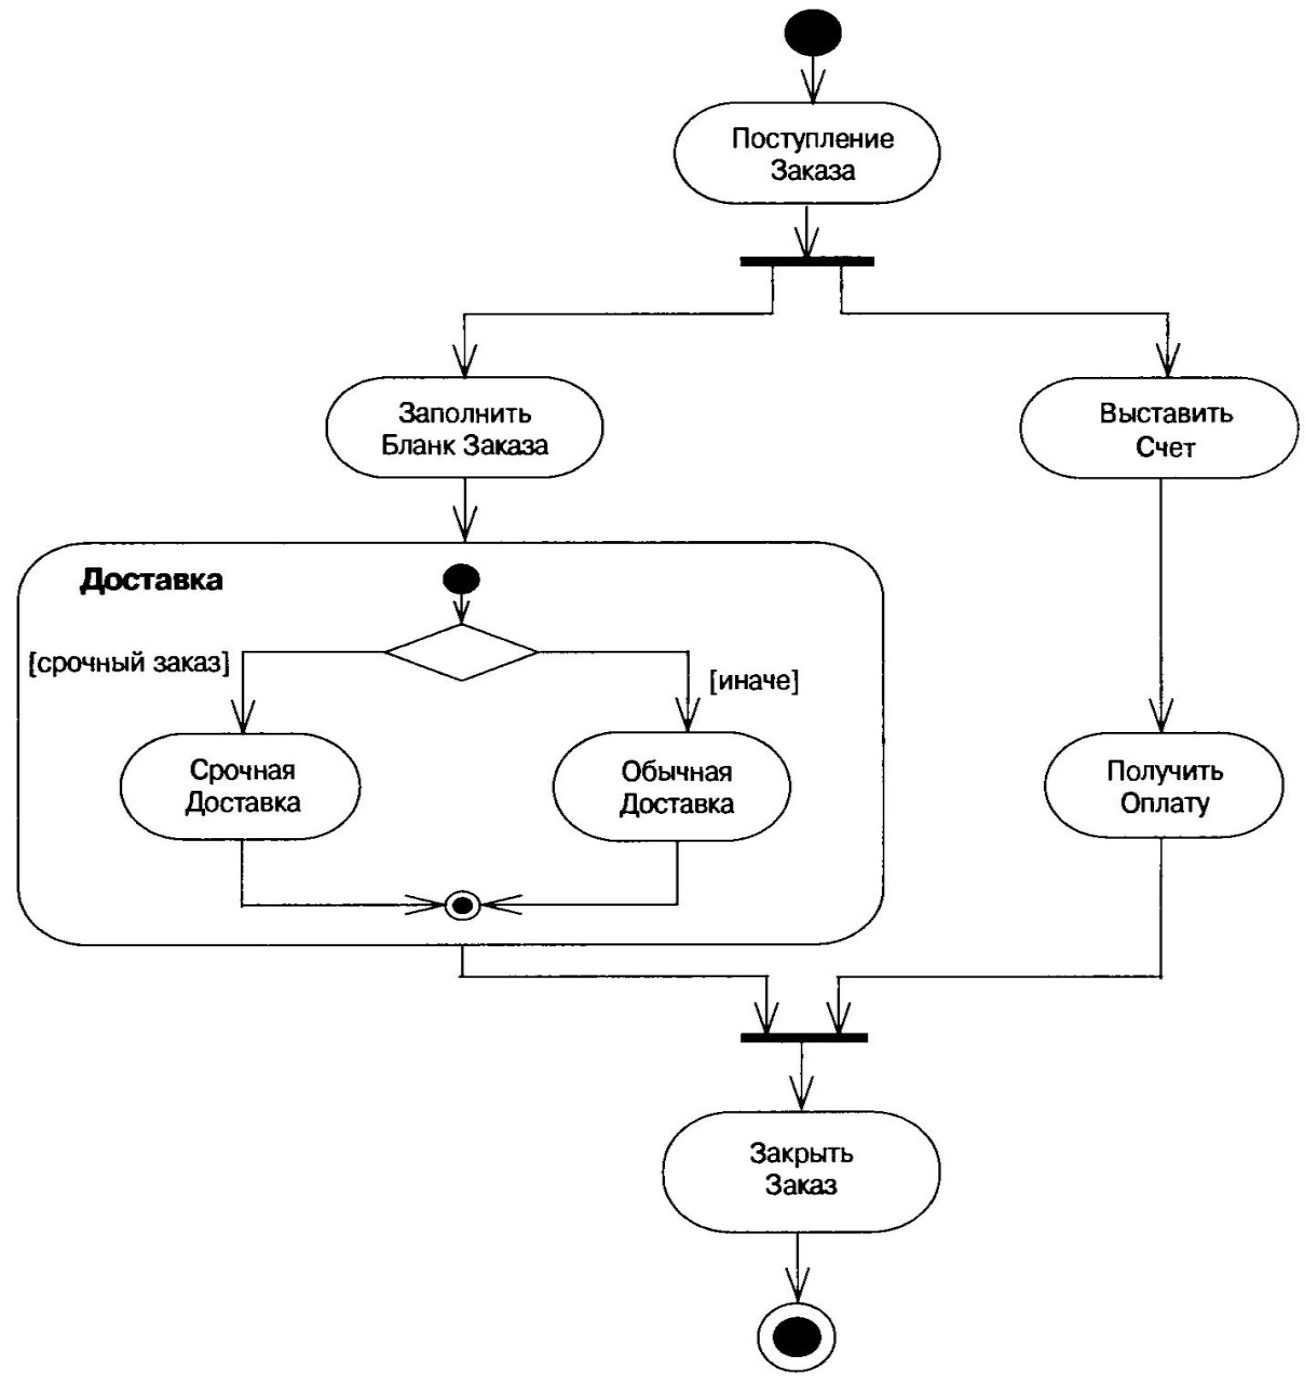
\includegraphics[width=0.7\textwidth]{activitySubdiagrams.png}
\end{center}

На этих диаграммах могут рисоваться ещё разные вещи, например, посылка и приём сигнала (но вам оно пока не нужно, потому что параллельные программы мы пока не писали), сигналы таймера, исключения, разделы (или дорожки), структурные узлы, задающие циклы, участки параллельного исполнения и т.д. Следует отметить, что диаграммы активностей --- одно из немногих мест в UML с более-менее чётко заданной семантикой, так что по таким диаграммам можно генерировать исполняемый код. Однако же, обычно для генерации кода и исполнения используются не диаграммы активностей, а диаграммы конечных автоматов.

\section{Диаграммы конечных автоматов}

Диаграммы конечных автоматов (или диаграммы состояний, state machine diagrams) служат для спецификации поведения классов, в отличие от диаграмм активностей, которые специфицируют поведение конкретного метода. На диаграмме изображаются все возможные состояния объекта, а также изменения состояния объекта, которые происходят вследствие влияния неких внешних событий на этот объект. Выглядит диаграмма так:

\begin{center}
	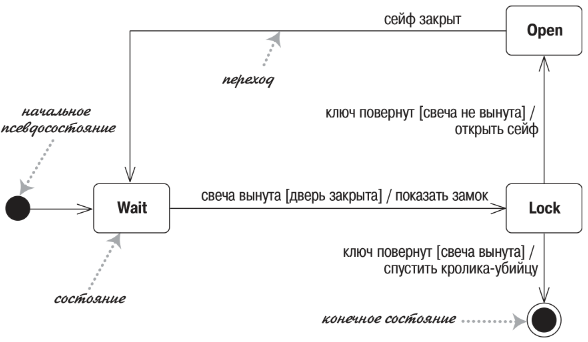
\includegraphics[width=0.7\textwidth]{stateTransitionSyntax.png}
\end{center}

На диаграмме изображены состояния (state) и переходы (transition). Переходы имеют метки, в формате ``триггер-идентификатор [защита]/активность'', все они необязательны. Триггер-идентификатор указывает, по какому событию может происходить переход, защита --- логическое условие, которое должно быть выполнено, чтобы переход состоялся. Активность --- что надо делать во время перехода. Тут может быть ссылка на диаграмму активностей. Активности могут писаться и прямо внутри состояния (они называются внутренними активностями), синтаксис там такой же, а работают они как переходы из состояния в себя с выполнением нужной активности. Состояния могут быть вложенными, есть возможность указать параллельные состояния, но как --- выходит за рамки лекции.

Заметим, что диаграммами автоматов (хотя и менее общими) мы пользовались в первом семестре, когда писали лексические анализаторы. Ещё следует обратить внимание на отличие диаграмм автоматов и диаграмм активностей (хотя бы потому, что диаграммы активностей выделили в отдельный вид диаграмм не с первых версий UML). В диаграммах активностей действия выполняются в узлах, а в диаграммах автоматов --- при переходах. Кроме того, как уже говорилось, диаграммы автоматов рисуются для всего класса, а активностей --- для каждого конкретного метода. Диаграмма автоматов более высокоуровневая, чем диаграмма активностей, однако, с её помощью удобно реализовывать только системы, хорошо выражающиеся в терминах конечных автоматов (те же лексические анализаторы). Впрочем, в ИТМО есть большая группа уважаемых людей (во главе с проф. Шалыто), полагающая, что диаграммы автоматов способны адекватно описать вообще любую систему, и они умеют делать даже визуальные отладчики диаграмм автоматов. Другие не менее уважаемые люди (Фаулер, например), впрочем, считают, что диаграммы автоматов не годятся для описания сложных систем взаимодействующих объектов.

\section{Диаграммы случаев использования}

Ещё одной часто используемой и весьма полезной диаграммой UML является диаграмма случаев использования (или прецедентов, use case diagram). Используются они на фазе анализа для определения и обсуждения функциональных требований к системе. На диаграмме описываются типичные взаимодействия между пользователями системы и самой системой. Анализ требований к системе обычно начинается с описания сценариев взаимодействия пользователя и системы. Например, делаем мы онлайн-магазин. Неплохо бы, чтобы там было можно купить товар. Опишем, как происходит покупка товара: ``Покупатель просматривает каталог и помещает выбранные товары в корзину. При желании оплатить покупку он вводит информацию о кредитной карте и производит платёж. Система проверяет авторизацию кредитной карты и подтверждает оплату товара тотчас же и по электронной почте''. Это один сценарий, если у нас есть постоянный клиент, для которого проверка информации о кредитной карте необязательна, появится другой сценарий. В любом случае, цель у пользователя одна --- купить товар. Вот множество сценариев, объединённое общей целью и называется случаем использования. В терминах UML пользователи называются актёрами (actor). Актёр представляет не конкретного пользователя, а роль, которую пользователь играет по отношению к системе --- один и тот же человек может выступать в двух ролях (например, админ онлайн-магазина сам может делать в нём покупки). Заметьте, что в роли актёра может выступать не только человек, но и другая система, внешняя по отношению к нашей, или другой компонент системы, если мы рисуем диаграмму случаев использования для компонента. 

Выглядит диаграмма так:

\begin{center}
	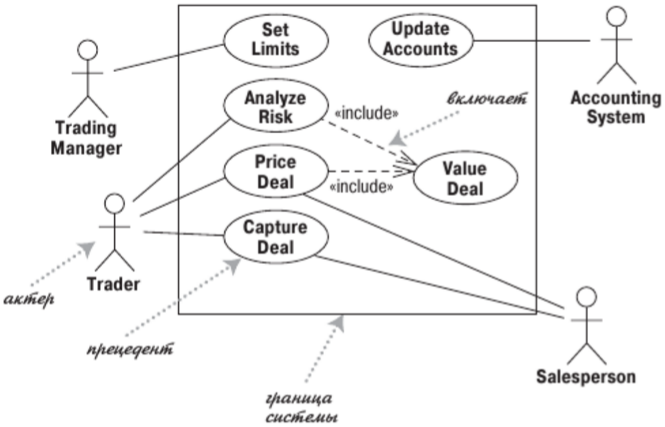
\includegraphics[width=0.7\textwidth]{useCaseDiagram.png}
\end{center}

Между случаями использования могут быть отношения обобщения (на самом деле, между актёрами тоже), отношения включения. Однако, умные люди рекомендуют не заморачиваться, а сконцентрировать внимание на текстовом описании случаев использования --- которое должно включать типичный сценарий взаимодействия в этом случае использования и возможные отклонения от этого сценария. С такой диаграммой и текстовыми описаниями вы будете чётко представлять, что вы хотите от системы. Например, для написания калькуляторов такое бы весьма сгодилось --- непродуманное поведение при нажатии на знаки арифметических операций приводило к забавным багам.

\section{Диаграммы компонентов}

К диаграммам, которые можно нарисовать и повесить на стенку, относятся, в частности, диаграммы компонентов. Диаграммы компонентов показывают различные компоненты системы и связи между ними. Что такое компонент --- вопрос сложный, о котором до сих пор спорят, но вполне можно считать компонент просто большой и обособленной частью системы (обособленность здесь, пожалуй, ключевое свойство). Компоненты полезно использовать вместе с диаграммами размещения (да, UML допускает смешивать нотации разных видов диаграмм, но надо использовать это осторожно). Выглядит это как-то так:

\begin{center}
	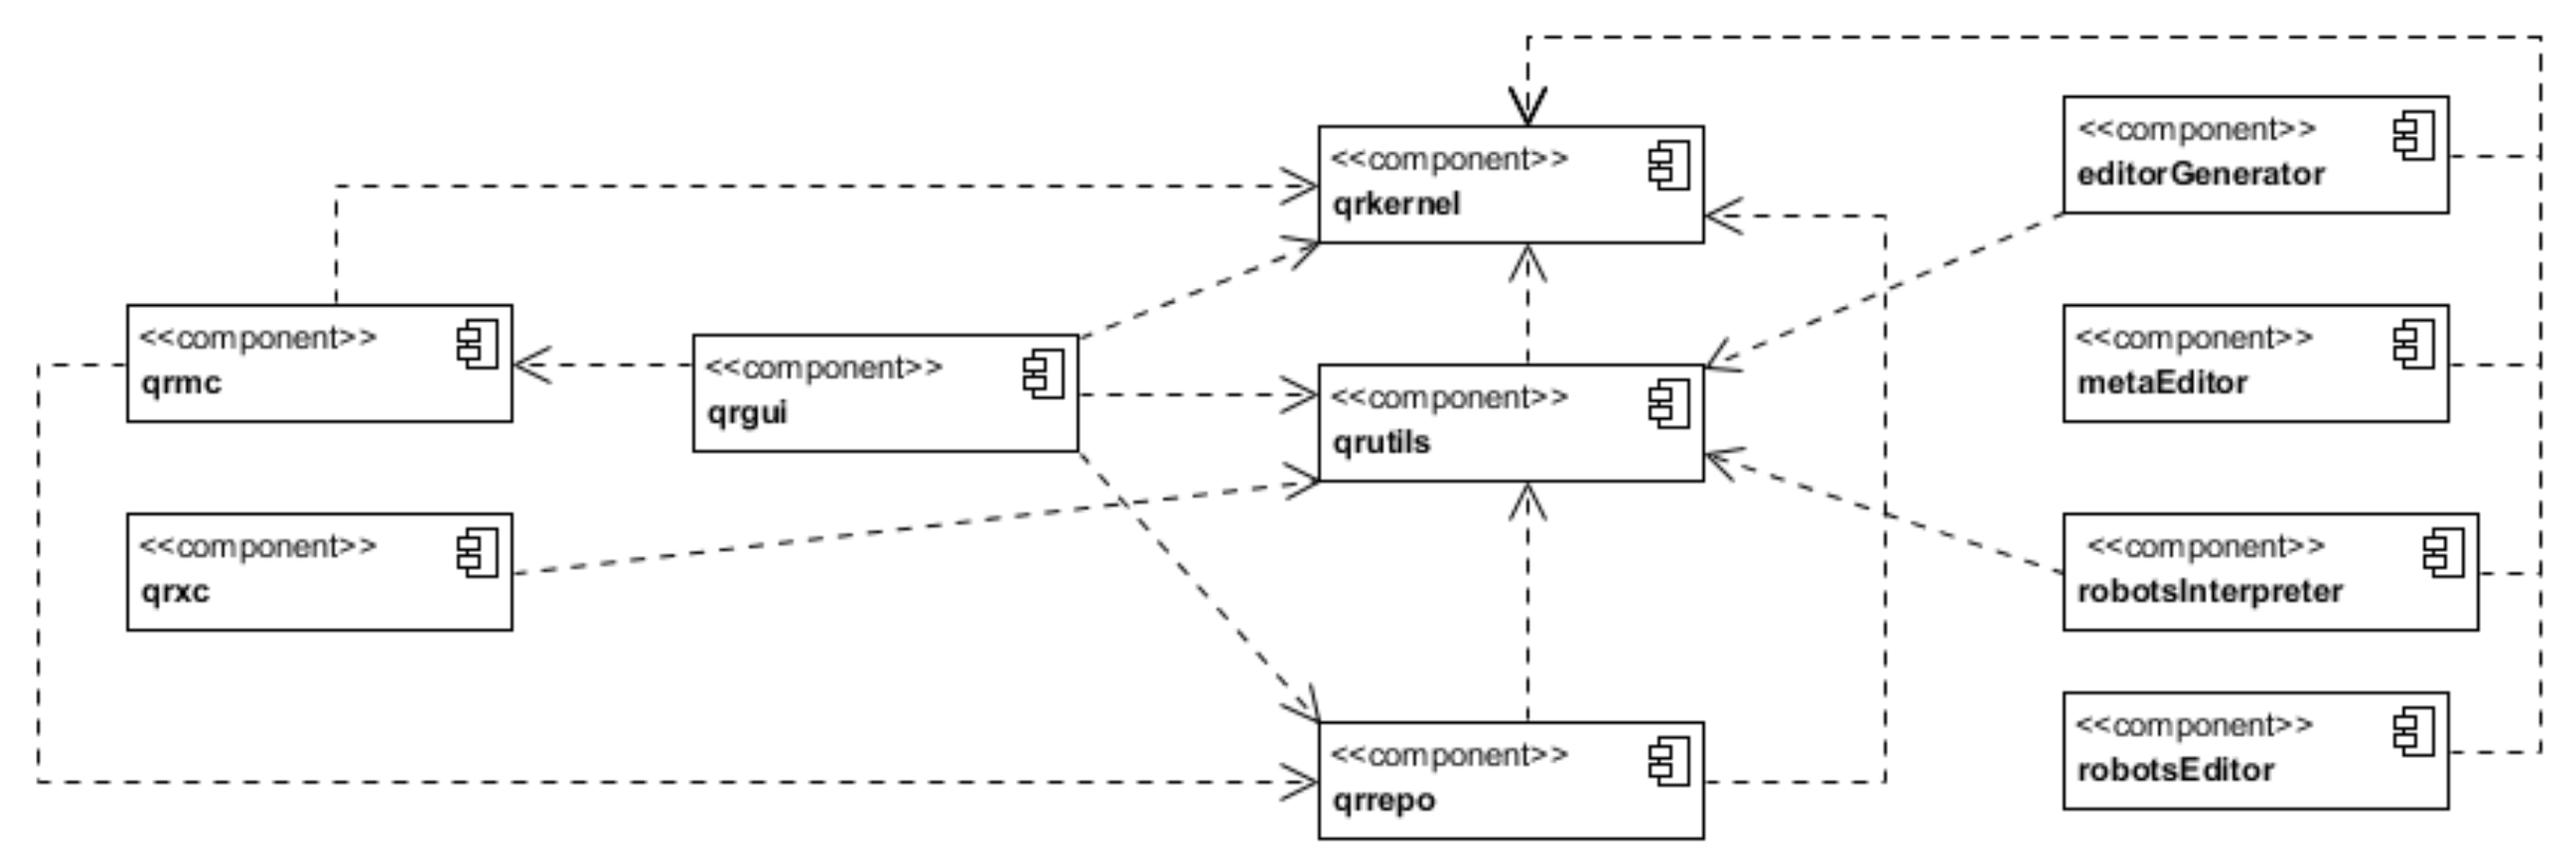
\includegraphics[width=0.95\textwidth]{componentDiagram.png}
\end{center}

Компоненты раньше использовались для представления физических частей системы --- .dll, например. Теперь для этого используется другая нотация, так что можно использовать диаграммы компонентов для рисования высокоуровневой архитектуры системы.

\end{document}
